\documentclass[uplatex, titlepage]{jsarticle}
\usepackage[dvipdfmx]{graphicx}
\usepackage{float}

\title{R2.移動電話の加入台数を予測する}
\author{C0118005 A3 秋本 遥基}
\date{}

\begin{document}
\maketitle

\section{目的}

   本レポートでの目的を移動電話の加入台数について、過去データに基づく分析を行いその動向をまとめることである。
過去データの範囲は具体的に2013年度末から2016年度末である。
これによる推定結果に基づいて今後の移動電話の加入台数についての考察を行った。

\section{方法と結果}

   以下に実験の方法と結果を示す。データの測定と推定は本来同節にすべきだが、規定の書式に基づいた。
各用語について、携帯電話、PHS、無線呼び出し、とあるがこれらを総称して移動電話と呼ぶ。
本レポートでは携帯電話を1979年に自動車電話として登場し現在最も多くの利用者が使用している電話機を指す用語とし、
PHS、無線呼び出しをそれぞれ携帯電話に含まないものとした。
またPHSを移動電話、無線呼び出しを文字表示に限ったi液晶端末の区切りとした。
実験2で用いたロジスティック曲線はロジスティック方程式、ロジスティック関数によって導出される曲線である。
主に生物の個体数モデルなどに適応される。限られた資源の環境においての増殖などに用いられるため、これを用いた。

\subsection{実験1}

   過去データの収集にあたり、電気通信事業者協会のwebページを参考にした。\cite{data}\\
また、移動電話加入台数の表より移動電話加入台数の推移のグラフを作成した。


\begin{figure}[H]
  \centering
    \begin{tabular}{c}
      \begin{minipage}{0.5\hsize}
        \begin{center}
          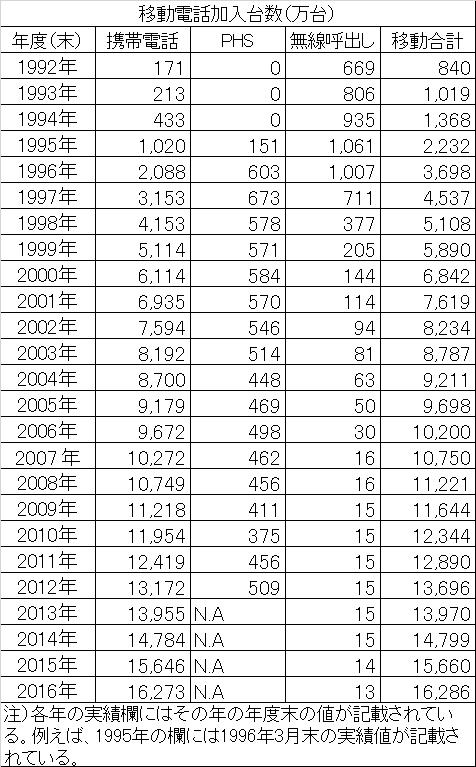
\includegraphics[scale=0.7]{./re2/f11.png}
          \caption{移動電話加入台数}
          \label{fig:table1}
        \end{center}
      \end{minipage}
      \begin{minipage}{0.5\hsize}
        \begin{center}
          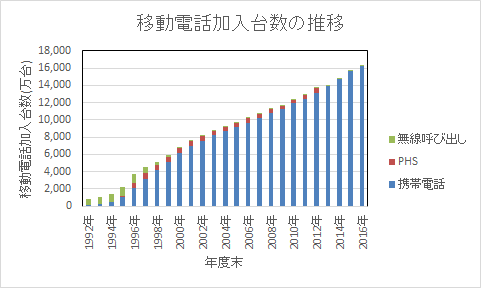
\includegraphics[scale = 0.9]{./re2/f1.png}
          \caption{移動電話加入台数の推移}
          \label{fig:graphicx1}
        \end{center}
      \end{minipage}
    \end{tabular}
\end{figure}


以上より、加入台数増加分を計算して、表をまとめた。この数値は移動電話加入台数での$該当年度-前年度$により計算した。
これについての表とグラフを以下に示す。


\begin{figure}[H]
  \centering
    \begin{tabular}{c}
      \begin{minipage}{0.5\hsize}
        \begin{center}
          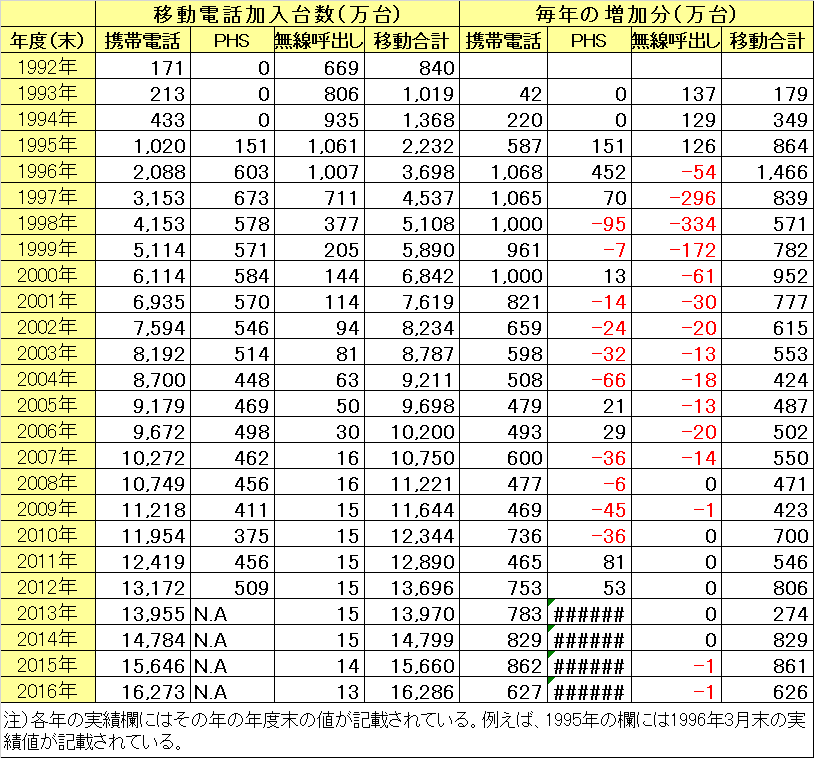
\includegraphics[scale = 0.5]{re2/f3.png}
          \caption{加入台数増加分の計算}
          %\hspace{1.6cm}
          \label{fig:table2}
        \end{center}
      \end{minipage}
      \begin{minipage}{0.5\hsize}
        \begin{center}
          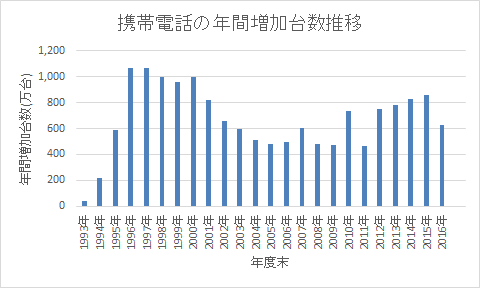
\includegraphics[scale = 0.9]{re2/f4.png}
          \caption{携帯電話の年間増加台数推移}
          \label{fig:graphicx2}
        \end{center}
      \end{minipage}
    \end{tabular}
\end{figure}


以上の数値から移動電話の加入台数の伸び率の推移の数値を計算した。これは$(該当年度-前年度)/前年度$で算出した。
これについての表とグラフを以下に示す。


\begin{figure}[H]
  \centering
    \begin{tabular}{c}
      \begin{minipage}{0.5\hsize}
        \centering
          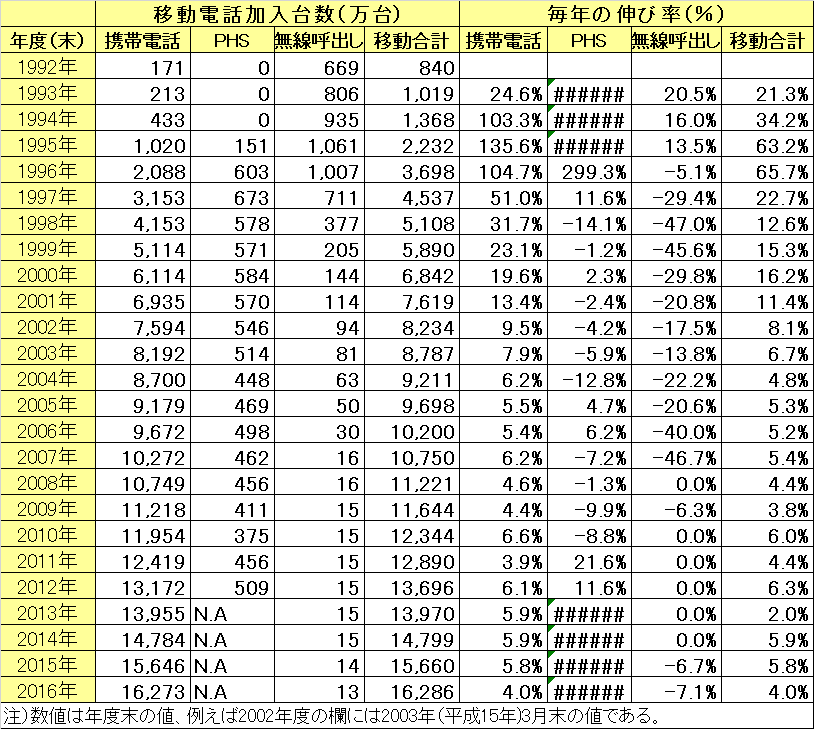
\includegraphics[scale = 0.5]{re2/f5.png}
          \caption{加入台数年度別伸び率}
        \label{fig:table3}
      \end{minipage}
      \begin{minipage}{0.5\hsize}
        \centering
          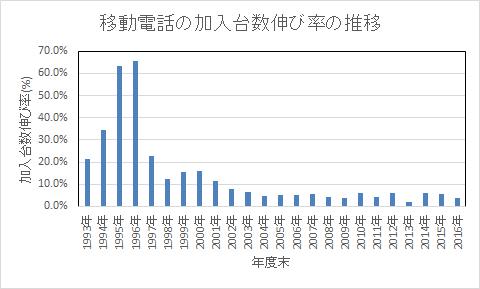
\includegraphics[scale = 0.9]{re2/f6.png}
          \caption{移動電話の加入台数伸び率の推移}
        \label{fig:graphicx3}
      \end{minipage}
  \end{tabular}
\end{figure}


結果として、移動電話の加入台数の伸び率は1995年年付近で全盛期を迎え、以降は安定した伸び率であった。
合計、伸び率から、観察した以降の年度も緩く増加傾向にあると推定される。
内訳としては2013年度以前ではPHSが300から500万台で安定している。以降有効数が見られない。
無線呼び出しに関しては近年の伸び率から、減少傾向にあると思われる。
携帯電話は伸び率から分かる通り、順調に加入台数が伸びている。
また、内訳からして2000年以降で安定した伸び率を見せているのは移動電話の中で携帯電話のみである。

\newpage
\subsection{実験2}

ロジスティック曲線について実験を行った。用いた式を示す。

\begin{equation}
\mathrm{z}(x) & = & \frac{K}{1+exp(-a-bx)}
\end{equation}

これにより生成したグラフ、及び使用した各値を示す。


\begin{figure}[H]
  \centering
    \begin{tabular}{c}
      \begin{minipage}{0.5\hsize}
        \centering
          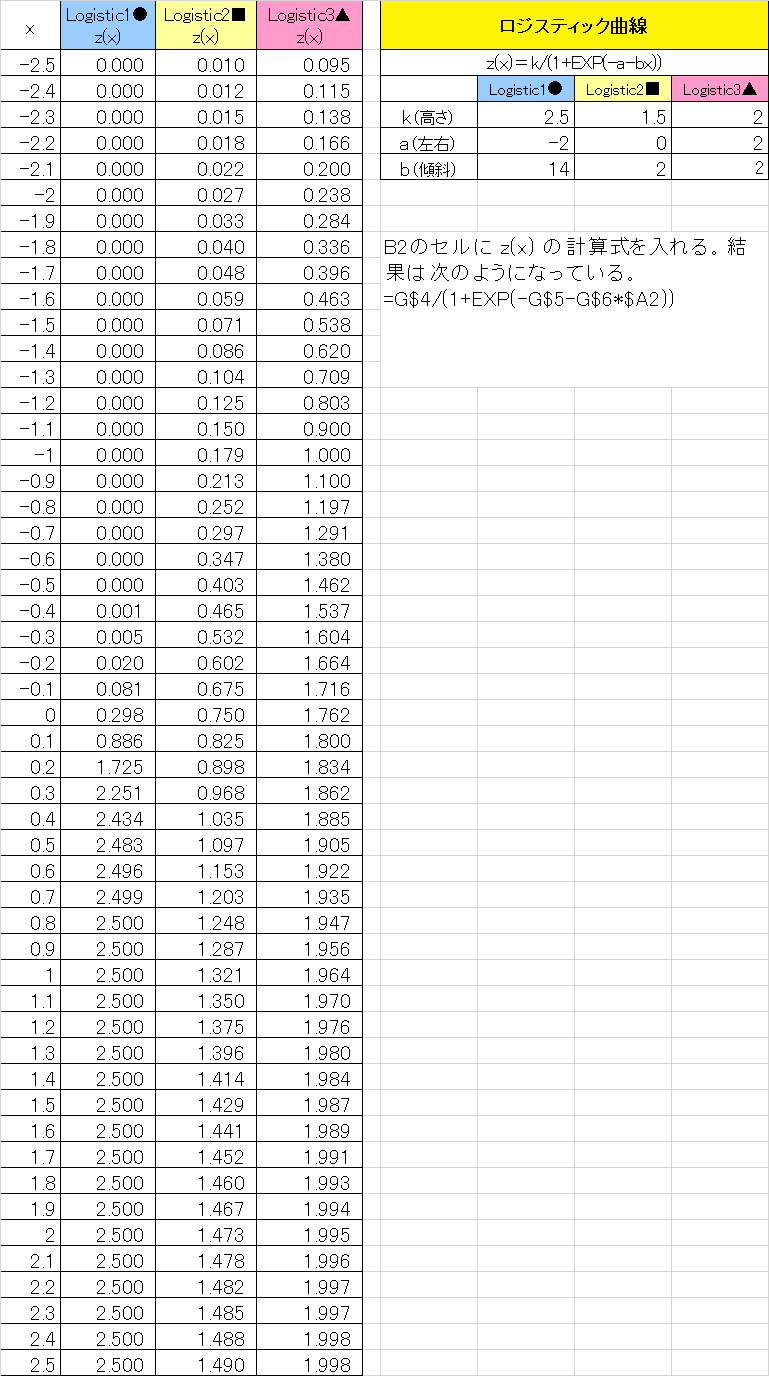
\includegraphics[scale = 0.5]{re2/f7.png}
          \caption{ロジスティック曲線の設定}
        \label{fig:table4}
      \end{minipage}
      \begin{minipage}{0.5\hsize}
        \centering
          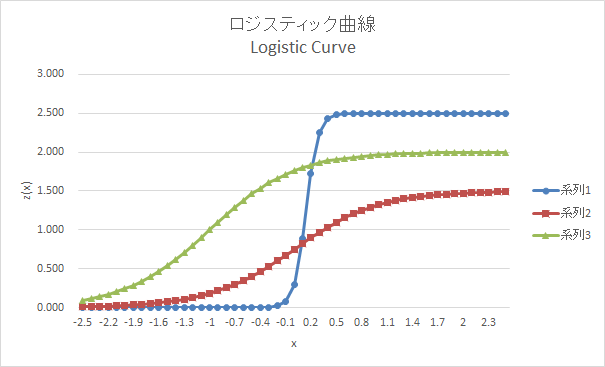
\includegraphics[scale = 0.9]{re2/f8.png}
          \caption{ロジスティック曲線}
        \label{fig:graphicx4}
      \end{minipage}
  \end{tabular}
\end{figure}


次に移動電話加入台数推移について、ロジスティック曲線のフィッティング作業を行った。
これはmicrosoft社の表計算ソフトExcelのソルバー機能によって求めた値である。
結果を次に示す。


\begin{figure}[H]
  \centering
    \begin{tabular}{c}
      \begin{minipage}{0.5\hsize}
        \centering
          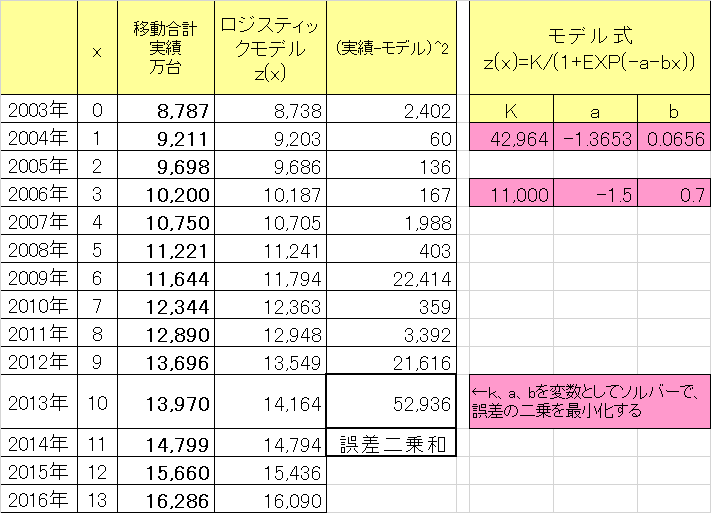
\includegraphics[scale = 0.5]{re2/f9.png}
          \caption{ロジスティック曲線によりフィッティングを行うワークシート}
        \label{fig:table5}
      \end{minipage}
      \begin{minipage}{0.5\hsize}
        \centering
          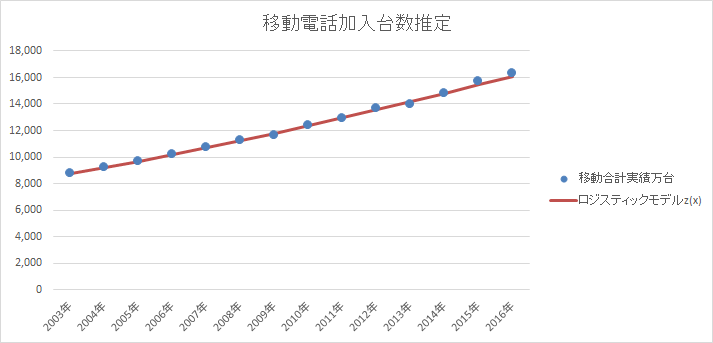
\includegraphics[scale = 0.8]{re2/f10.png}
          \caption{移動電話加入台数推定}
        \label{fig:graphicx5}
      \end{minipage}
  \end{tabular}
\end{figure}


結果として、ロジスティック曲線のフィッティング作業によって各年度の推定値がわかった。
各値に可能な限り近づくようにグラフが生成され、十分に説得力のある推定値を出すことができた。

\section{考察}

   ロジスティック曲線と過去年度の移動電話の加入台数より、加入台数の伸び率により各表及びグラフを作成した。
方法と結果でも述べたとおり、ロジスティック曲線を用いることによってただ最小二乗法で数値を得るよりも具体性があり、なおかつ説得力のある数値であると確信した。
ロジスティック曲線の起源を調べると、生物の増加データに対して適応させるためのロジスティック方程式及びロジスティック関数とあったので、
野生生物の増減のデータ(肉食獣と草食獣の混在した場でのデータ)などに適応させて、数値の未来予測などするのも良いとも思われる。
また、今回のように消費者の有効獲得数を得たい場合、今回の方法、手順をテンプレートとして用いても様々な予測が可能になると考えられる。
移動電話全体では、携帯電話が最も大きなものになっていたが実際に日本市場で取引されている各メーカー別の数値を使うのにも興味を抱いた。

\begin{thebibliography}{99}
\bibitem{data}https://www.tca.or.jp/

  \end{thebibliography}
\end{document}
